\documentclass{neu_handout}
\usepackage{url}
\usepackage{amssymb}
\usepackage{amsmath}
\usepackage{marvosym}
\usepackage{graphicx}
\usepackage[pdftex]{graphicx}
\usepackage{subfigure}
\usepackage{listings}
\usepackage{color}

\definecolor{dkgreen}{rgb}{0,0.6,0}
\definecolor{gray}{rgb}{0.5,0.5,0.5}
\definecolor{mauve}{rgb}{0.58,0,0.82}

\lstset{frame=tb,
  language=Python,
  aboveskip=3mm,
  belowskip=3mm,
  showstringspaces=false,
  columns=flexible,
  basicstyle={\small\ttfamily},
  numbers=none,
  numberstyle=\tiny\color{gray},
  keywordstyle=\color{blue},
  commentstyle=\color{dkgreen},
  stringstyle=\color{mauve},
  breaklines=true,
  breakatwhitespace=true,
  tabsize=3
}

\graphicspath{ {images/} }
\everymath{\displaystyle}

% Professor/Course information
\title{Classifying High-Resolution Brain Scans using Apache Spark}
\author{Asha Chen-Phang, Emily Dutile, Nate Otenti, Tristan Sweeney}
\date{April 2018}
\course{EECE 5644}{Pattern Recognition and Machine Learning}

\begin{document}

\section*{1 Introduction}
Being in the multi-core and machine learning era, it is important for our machine learning algorithms to take advantage of the potential speed up through the use of paralleling tasks on multi-core computers and distributed systems. With an interest in processing a massive image dataset, performing feature engineering and using well-known industry solution for faster computation, the group used Apache Spark, a processing model for analyzing big data, to analyze the speed up of machine learning algorithms for foreground-background classification in high-resolution brain scans. With the dataset, we performed preprocessing, feature extraction, model implementations in python using sklearn in a single-processor solution, and model implementations in scala on top of Apache Spark using MLlib to analyze time and processing efficiency in a parallel processing program upon distributed data. In a single machine environment, we experimented with SVM, KNN, and Random Forest. In our parallelized environment, Random Forest was implemented to analyze the model and training phase with parameter tuning in comparison to a single processor environment. The Apache Spark environment was created on an Amazon EMR cluster, leveraging the EMR file system (EMRFS) to access data in Amazon S3.\\

The dataset we are working with comes from a group of scientist who have an interest of turning high-resolution brain scans, as seen in the left figure \ref{fig:left}, into a graph representing nerve connections indicated by the bright lines. The original image is 3-dimensional. For better intuition the 2-dimensional projection on the X-Y plane is shown. As you can see, the image is noisy but the axons, which are the lines going across the image, are clearly visible. To improve the quality of algorithms that automatically trace these axons in an image, each pixel was classified as either foreground (belongs to an axon) or background (does not belong to an axon). The group of scientists manually traced the axons. The traced data looks like the figure on the right\ref{fig:right}, where white indicates foreground and black indicates background.\\

\begin{figure}[h]
\centering
{
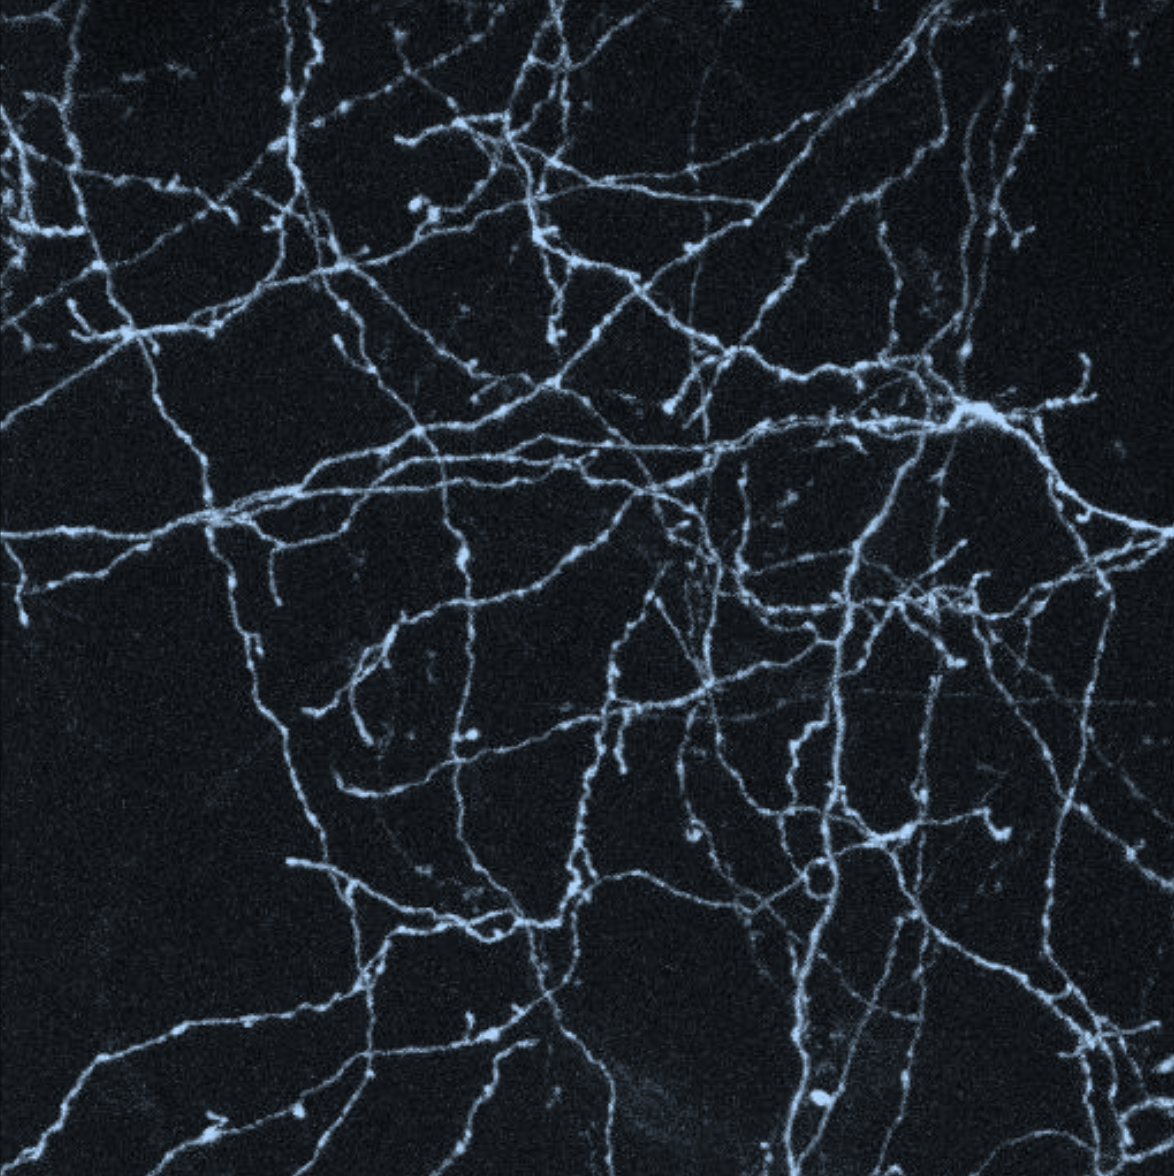
\includegraphics[width=0.2\linewidth]{image1}
\label{fig:left}
}
{
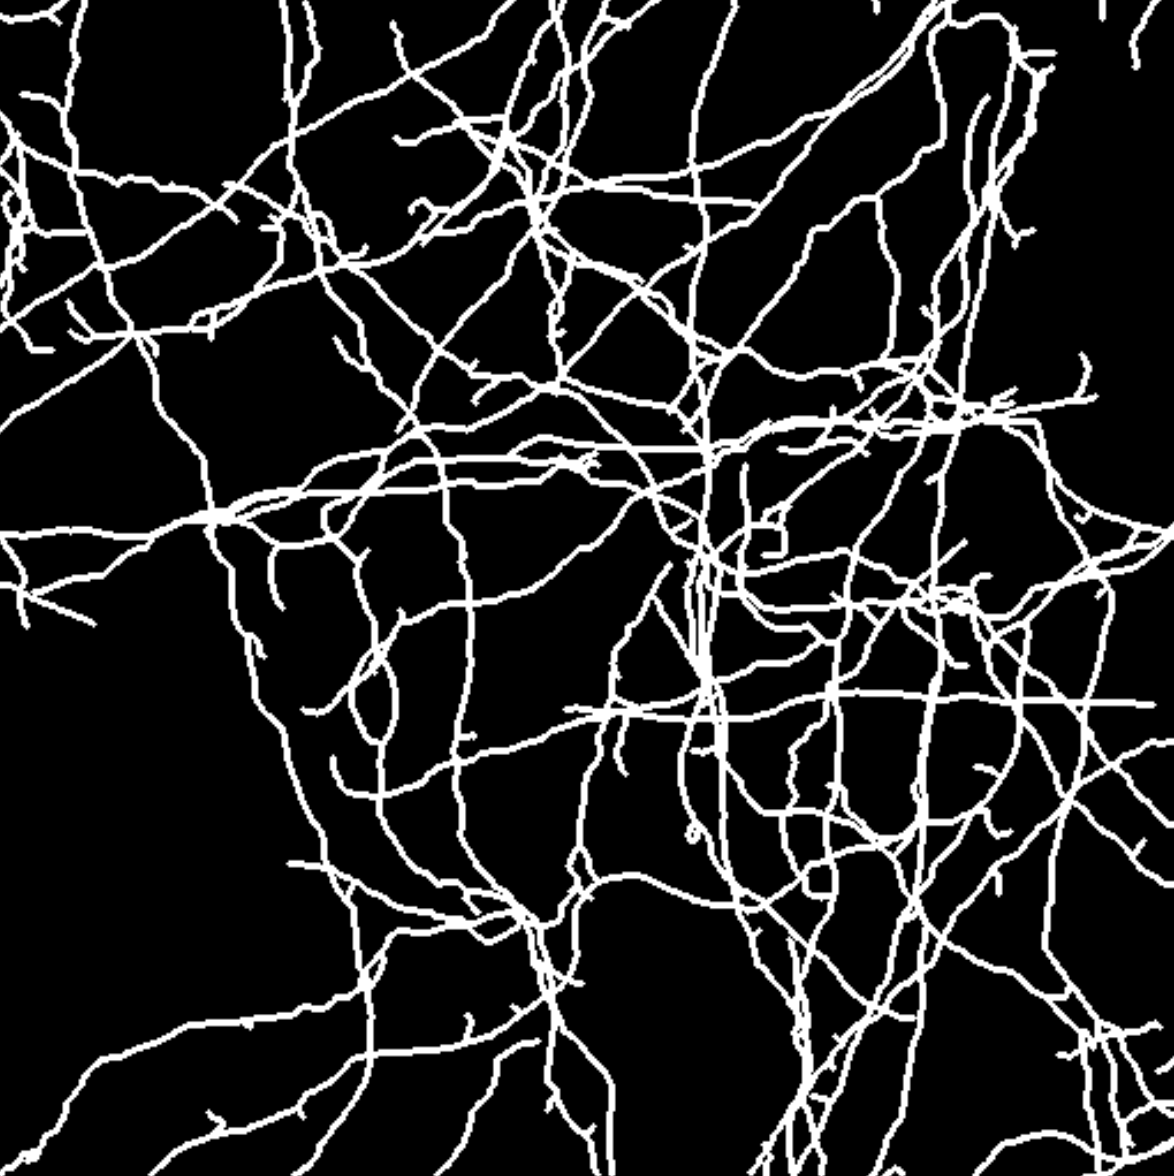
\includegraphics[width=0.2\linewidth]{image2}
\label{fig:right}
}
\end{figure}


Using the manually traced image, the labeled data was generated as follows:
\newenvironment{myitemize}
{ \begin{itemize}
    \setlength{\itemsep}{0pt}
    \setlength{\parskip}{0pt}
    \setlength{\parsep}{0pt}     }
{ \end{itemize}                  } 

\begin{myitemize}
  \item Select a pixel (i, j, k) in the image.
  \item Extract a neighborhood vector centered around (i, j, k).
  \item Extract the label of (i, j, k) from the trace. Here 1 indicates foreground; 0 indicates background.
  \item  Save the record as the neighborhood vector, followed by the label.
\end{myitemize}

Assuming pixel (i=10, j=10, k=10) was selected and we are working with a neighborhood of size 3x3x3, these 27 pixels would be stored as a vector n with 27 elements, where n[0] stores the brightness value of
pixel (9, 9, 9), n[1] the brightness of (9, 9, 10), n[2] of (9, 9, 11), n[3] of (9, 10, 9), n[4] of (9, 10, 10), and so on. The labeled data set contains neighborhoods of size 21x21x7, which was recommended by the domain experts.\\

\subsection*{1.1 The Data}
The dataset\footnote{\url{https://drive.google.com/drive/u/0/folders/1EJBgJFmp-FQf2czw9LGImoOhEO2OvOoo}} is composed of several labeled csv files, each consisting of rows that contain an input vector of 21x21x7
brightness values (intensity) from a 3D image, together with the center pixel's foreground-vs-background label. The last value is the label for the whole image. On each line there are 21*21*7+1 values. Each image, which is a csv file, is roughly 6.5 GB. The labeled data from images 1, 2, 3, 4, and 6 are used to train the most accurate model for predicting the labels in image 5 of the datasets. In the final evaluation set, there are nearly 0.0057\% foreground and 99.99943\% background pixel. For classification accuracy, a high value does not necessarily mean the model is performing well. In our case, the ``dumb'' model that always predicts label 0 for every input will have 99\% accuracy, so any model achieving less than 99\% would not be beating the dumb model. \\

Using the standard way of training and testing a classification model, the labeled data is partitioned into 3 separate sets: training, validation and test data. Although uniform random partitioning into training and validation data often works well, for this particular data set it is not sufficient. Assume we have two labeled records with centers (x,y,z) and (x+1, y+1, and z+1), in this case, uniform sampling could assign (x,y,z) to training and (x+1, y+1, and z+1) to the validation data. The two neighborhoods and labels of the two pixels are highly correlated. The model would overfit to the training data and give overly optimistic validation accuracy from the correlations. To ensure independent training and validation, partitioning by image is performed.\\

\section*{2 Related Works}
Being in the big data age, datasets are rapidly growing in size and complexity. Due to this, cloud computing architectures and solutions are becoming more pervasive and machine learning is also becoming a vital component of these large-scale data processing pipelines. Under this umbrella, exploratory analysis, feature engineering, machine learning, and model evaluation are all critical components to the distribute machine learning solution. Since many machine learning techniques are computationally expensive, this makes them ideal candidates for parallelization. However, these methods are usually complex, so implementing a parallelized solution is often challenging.\\

Apache Spark is a well known open source framework that is becoming more readily used within industry as a cluster computer system that excels in scaling machine learning tasks, including its open-source distributed machine learning library as a standard component, MLlib \cite{mllib}. MLlib contains algorithms for classification, regression, collaborative filtering, clustering, and decomposition. Apache Spark is known for its speed it comparison to Hadoop MapReduce, running programs up to 100x faster in memory or 10x faster on disk. For programmers, it can be used to quickly write applications in either Scala, Java, or Python. Spark SQL, another Spark component, is also available to easily extract data from sources, such as Apache Hive. Since Spark has named its as a general purpose big data platform, its easy to run in standalone mode locally, on YARN or Amazon's EC2, and it also reads from HDFS, Amazon's S3, and HBase. Industry technology leaders are leading towards Spark MLlib due to its scalability, performance, user friendly APIs, and its other components.\\

The model training phase and model use (prediction) phase of decision trees are possible targets for parallelization. Decision trees are ``easier'' to parallelize in comparison to many other classification models because of their tree structure.

With respect to the dataset being used, the other interesting task at hand is dealing with imbalanced data and since our machine learning algorithms usually assume that the number of items per class is roughly similar. As Bartosz Krawczyk explains in \textit{Learning from Imbalanced Data: Open Challenges and Future Directions} \cite{Krawczyk}, our systems that learn from imbalanced data often have a hard time overcoming these biases without an overly complex system. Over the past several years, ensemble methods are widely used in order to handle class imbalance due to its successful approaches of Boosting and Bagging. Although accuracy is a very common metric for many traditional machine learning applications, in practice it is often observed that 0 is the value of the recall for the minority class. Due to this, other metrics need to be considered, such as a confusion matrix in order to see better performance on the minority class \cite{imbalance}.

\section*{3 Methods}
Various models were evaluated in order to receive the highest accuracy of predictions on the high resolution brain scans\footnote{\url{https://drive.google.com/drive/u/0/folders/1EJBgJFmp-FQf2czw9LGImoOhEO2OvOoo}} such as Linear SVM, Nearest Neighbor, Decision Tree, Neural Net and AdaBoost. Different models were trained on a subset of the data: 100 random background samples and 100 random foreground samples. We observed that the decision trees, and the two ensemble methods were the ones that performed the best, so Random Forest become the focus since it is also available in MLlib. Random forests is a well-known ensemble method that's used to build predictive classification models. The model creates an entire forest of random uncorrelated decision trees to arrive at the best possible answer. Random Forest looks to reduce a correlation issue, a limitation to bagging trees, through choosing a subsample of the feature space at each split by using a stopping criteria for node splits to prune the trees. Exploration of multiple parameter combinations was explored to achieve the best possible accuracy. \\

\subsection*{3.1 Data Analysis and Feature Extraction}
To begin visualizing the data, we performed our analysis using Jupyter Notebooks, numpy, and matplotlib. To do so, we took one of the csv files, found the rows of the file that are labeled as 1, found the rows of the file that has 0 as the label, and generated a file with 100 ``foreground'' images and 100 ``background'' images (see Appendix \ref{fig:visualization}). Visualizing this subset of data increased our intuition on what were the important features to segregating samples from different classes.\\

Image pre-processing and feature extraction was performed with the hopes to reduce the sample size, and, consequently, be able to try more parameters as the training will be speed up (see Appendix \ref{fig:visualization} for the comparison of images of foreground sample and background sample). We looked at the distribution of the training data since we knew we were dealing with class imbalance on the validation/prediction data set (image 5) and found thresholds in order to avoid misleading accuracy metrics. The statistics on all of planes( xy, xz, yz ) slices for the two images led us to identifying important features along with a threshold to tell the difference between a foreground and background image. By looking at the images for foreground and background, we noticed that there were some obvious features that were highly correlated to the label such as the center pixel value - the center pixel value is usually high in a foreground image, and usually low in a background image. From this we decided not to train complicated models on the full image but to use the following features and consequently the feature vector for all 3 planes XY, XZ, YZ:

\begin{itemize}
\setlength\itemsep{0.2em}
\item center pixel value
\item average of a window of pixels around the center pixel (FFT slice mean)
\item number of pixels with intensity greater than a threshold (50)
\end{itemize}

In the application Pipeline (see Appendix \ref{fig:pipeline}) \textit{Feature Extraction} is our first job. It is in charge of reducing the dataset size from 6 GB per image to ~65 MB per image. This is one job per image. This piece has been implemented as a map only job and has to be executed in every sample data (train, test, validation). \\

From our data analysis we performed a classification comparison of several classifiers on a smaller sample of the dataset through cross validation to gain a better sense of the nature of the decision boundaries of different classifiers with respect to the dataset. In Appendix D, the classifier comparison can be viewed along with the classification accuracy on the test set in the lower right. The test set contained a balanced scenario with 100/100 samples, proving that the Random Forest had the best accuracy with a 60/40 train/test sample using the feature vector without parameter tuning. According to our previous research on dealing with imbalanced data, these results aligned.

\subsection*{3.2 Parameter Tuning}

Hyperparameter optimization was performed. Changes of parameters controlling partitioning affected performance and accuracy. The parameters that we tweaked and set in our model were the following:

\begin{itemize}
\setlength\itemsep{0.2em}
\item Maximum depth of tree: splits for all trees in the forest. Higher values can lead to overfitting which decreases accuracy and increases run time of the phases. We observed the number of tasks increasing when increasing the depth.
\item Number of tress: automatically train trees until performance is maximized or specify the number of trees. We saw a correlation between increasing the number of trees and our performance in scaling.
\item Maximum bins: increasing this allows the algorithm to consider more split candidates and make fine-grained split decisions but it increases computation and communication. We saw better results but longer run times by increasing. We observed an increase in metadata shuffle when increasing bins during the phase of Random Forest training.
\item Impurity: gini was used since it does not require computing logarithmic functions like entropy (less expensive) and online reports had shown that this measure has a small effect on performance.
\end{itemize}

\subsection*{3.3 Parallel Processing}
Our distributed parallel application pipeline (see Appendix \ref{fig:pipeline}) runs on AWS EMR. First, preprocessing was 1 job per image. Next, pre-processing transforms 6GB images on 65MB image. The training images are fed into the Random Forest Model to train. The image is persisted, which is a job that shuffles the data depending on the parameters. The classification job has a persisted model and it receives only the image that we want to classify. Since we intentionally made our feature vector small to help with class imbalance and performance, we didn’t see a lot of scaling during this phase (firing up more than 4 worker machines was not necessary).

\section*{4 Results}

As we learned through our readings and research, accuracy is not the best metric to select the best model, as it does not attribute the right importance to the minority class with respect to the dataset. However, we did use it as a scoring metric since we had an available file with the true results of image 5 to compare to in order to see if we beat the baseline after complete analysis, exploration and implementation. We also used confusion matrices to better analysis the results as recommended\cite{imbalance}.

\subsection*{4.1 Parallel System}
Table \ref{tab:parameters-runtime} shows the results of different Random Forest parameters on model accuracy. In our best model run on AWS, 10 machines with 40 partitions were used on the data in the training phase. In the prediction phase, only 4 machines were used.

\begin{table}[h!]
\centering
 \begin{tabular}{||c c c c c||} 
 \hline
Run time (mins) & Depth & Bins & Trees & Accuracy \\ [0.5ex] 
 \hline\hline
8.47  & 3  & 256 & 50 & 0.99718 \\
11.67 & 5  & 256 & 50 & 0.99730 \\
30.50 & 10 & 256 & 50 & 0.99759 \\
69.80 & 15 & 256 & 50 & 0.99761 \\
 \hline
27.77 & 10 & 32  & 50 & 0.99703 \\
27.83 & 10 & 64  & 50 & 0.99731 \\
29.50 & 10 & 128 & 50 & 0.99747 \\
33.87 & 10 & 512 & 50 & 0.99760 \\ 
 \hline 
5.80  & 4 & 256 & 25  & 0.99729 \\
8.47  & 4 & 256 & 50  & 0.99725 \\
30.23 & 4 & 256 & 100 & 0.99724 \\
\hline
\hline
22.8 	& 15  & 512 & 50 & 0.99768 \\[1ex] 
 \hline
 \end{tabular}
 \caption{Parameters Explored for Random Forest} \label{tab:parameters-runtime}
\end{table}

As we can see in the table above, increasing the depth, number of trees, and max bins increased the run time but also improved accuracy leading us to select depth of 15 and number of bins (discretization of the continuous features) as 512. When taking into account the number of trees, there was no gain beyond the point of 50 trees, for this reason, 50 was the selected metric.\\

The Confusion matrix \ref{fig:confusionmatrix} shows comparison between proposed baseline and best model accuracy. As it can be observed by the bold numbers in black and green, for the current testing set (the entire image 2 sample data), our model beats the baseline.

\begin{center}
\begin{figure}[!h]
\centering
  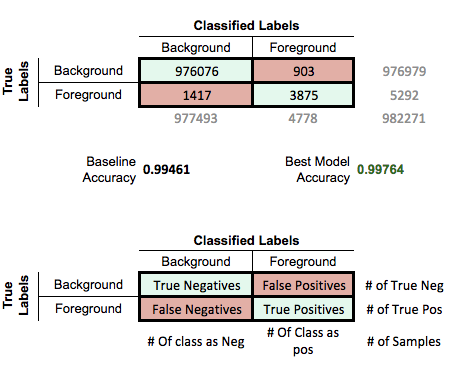
\includegraphics[width=0.5\linewidth]{confusionmatrix}
  \label{fig:confusionmatrix}
\end{figure}
\end{center}

The running time and speed up results for the model training and prediction phase on a single machine and Apache Spark are show below:

\subsubsection*{4.1.1 Model Training}

The following table shows that there is a a good speedup on running time when we scaled from 2 workers to 10 worker machines. Taking in consideration that 50 decision trees are being trained in the selected model, and that MLLib implements parallel tasks based on the number of trees and splits of data, it makes sense that the training job scales well with the increase of the number of available cores (workers* core/worker) up to the number of trees. But, beyond this point, the speedup gain stagnates which can be observed by the running time values of 10 (40 cores) and 19  workers (76 cores). 

\begin{figure}[!htb]
\begin{center}
 \begin{tabular}{||c c ||}
 \hline
Workers & Running Time (seconds) \\ [0.5ex] 
 \hline\hline
  2 & 2924  \\ 
  \hline
 10 & 582  \\ 
  \hline
 19 & 524  \\ [1ex] 
 \hline
\end{tabular}
\end{center}
\end{figure}

\begin{center}
$Speed up(x,y)$ = running time on $x$ machines / running time on $y$ machines

$Speed up(3,10) = 5.02$

$Speed up(3,19) = 5.58$
\end{center}

\subsubsection*{4.1.2 Model Prediction}

The table bellow show the running time for classification of the validation dataset with respect to the number of machines. During this job we have set the number of partitions to be equal to the number of available cores on our system. It is interesting to note that this job scales well until we reach 4 worker machines (16 cores). After this point, the application does not scale well and plateau at $~2.80$ speedup if compared to the running time of 1 machine. Inspecting the possible causes indicate that there is a non-negligible overhead when splitting and and using chunks of data smaller then $65/(4\times 4)=4MB$, which corresponds to:

$$ChunkSize = ValidationDataSize/(NofWorkers \times NofCores)$$

\begin{center}
 \begin{tabular}{||c c ||} 
 \hline
Workers & Running Time (seconds) \\ [0.5ex] 
 \hline\hline
 1 & 240  \\ 
 \hline
 2 & 160  \\ 
 \hline
 4 & 88  \\ 
 \hline
 8 & 92  \\ 
 \hline
 10 & 82  \\  [1ex] 
 \hline
\end{tabular}
\end{center}

\begin{center}
$Speed up(x,y)$ = running time on $x$ machines / running time on $y$ machines

$Speed up(1,4) = 2.727$

$Speed up(1,10) = 2.92$
\end{center}


\subsection*{4.2 Single Machine}

Small scale machine learning proved to be possible on a commodity laptop, given preprocessed data that had already undergone dimensionality reduction. Utilizing a python framework called SciKit-Learn (sklearn) we were able to train a random forest model on this preprocessed dataset with comperable accuracy. Such results can be seen tabulated below.

When attempting to perform fitting on the full dataset using sklearn the Jupyter notebook (the environment we were running in) consistently crashed, and never could make forward progress on training. It's easy to speculate that the crashing was due to us trying to load an excessive amount of data into memory, which caused Jupyter to crash. Running natively in a single python process, we found still that it was inpractical to load the entire dataset at once, as by the time it was loaded a significant amount of time had passed and in that time there was a nonzero chance that something could interupt training (laptop dieing/hibernating/crashing).

To be able to train a large classifier without blowing out the RAM capacity of our machine, we leveraged the ensemble nature of the random forest classifer and developed a tool on top of sklearn to partition the dataset and create seperate files for each tree in the forest, 

\begin{table}[h!]
\centering
 \begin{tabular}{||c c c||} 
 \hline
Model & Run time (mins) & Accuracy \\ [0.5ex] 
 \hline\hline
Random Forest & 22.8  & .99767   \\[1ex] 
 \hline
 SVM & 0  & 0 \\
\hline
KNN & 0  & 0 \\
\hline
 \end{tabular}
 \caption{Comparison of Models on Single Machine}
 \label{tab:accuracy-comparison}
\end{table}


\begin{figure}[h]
\centering
{
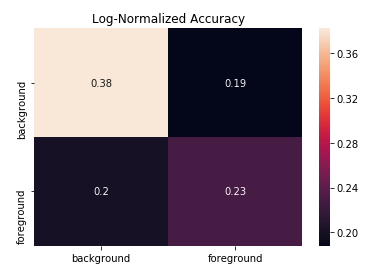
\includegraphics[width=0.4\linewidth]{rflocalgini}
\label{fig:rflocalgini}
}
{
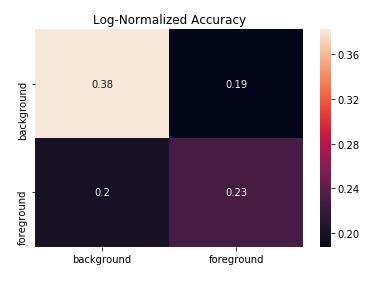
\includegraphics[width=0.4\linewidt h]{rflocalentropy}
\label{fig:rflocalentropy}
}
\end{figure}



\section*{5 Conclusion}
The purpose and motivation of our project was to take an interesting and complex image data set to perform the following: data analysis, feature extraction/pre-processing, parameter tuning, running and configuring an Apache Spark application in scala on AWS EMR, selecting and implementing an appropriate model, and analyzing the execution times between single machine runs and parallel runs. Datasets that suffer from class imbalance often result in bias or overly complex models, or made it nearly impossible to beat baseline accuracies of over 99\%. Our approach followed a mixture of recommended methods and ultimately beat the baseline of the validation data (image 5).


\newpage

\begin{thebibliography}{9}

\bibitem{andrewng} 
Map-Reduce for Machine Learning on Multicore,
\\\texttt{http://www.andrewng.org/portfolio/map-reduce-for-machine-learning-on-multicore/}

\bibitem{Krawczyk} Bartosz Krawczyk. \textsl{Learning from imbalanced data: open challenges and future directions}. November 2016, Volume 5, Issue 4, pp 221–232

\bibitem{imbalance} 
On the Class Imbalance Problem,
\\\texttt{http://sci2s.ugr.es/keel/pdf/specific/congreso/guo\_on\_2008.pdf}

\bibitem{amazonemr} 
Apache Spark - Amazon EMR,
\\\texttt{https://docs.aws.amazon.com/emr/latest/ReleaseGuide/emr-spark.html}

\bibitem{apachecheatsheet} 
Apache Spark Developer Cheat Sheet,
\\\texttt{https://mapr.com/ebooks/spark/apache-spark-cheat-sheet.html}

\bibitem{cross} 
Cross Validator Model,
\\\texttt{https://jaceklaskowski.gitbooks.io/mastering-apache-spark/content/spark-mllib/spark-mllib-CrossValidator.html}

\bibitem{compare} 
Classifier Comparison,
\\\texttt{http://scikit-learn.org/stable/auto\_examples/classification/plot\_classifier\_comparison.html}

\bibitem{ensembles} 
Classification by using Ensembles of Classifiers,
\\\texttt{https://grzegorzgajda.gitbooks.io/spark-examples/content/classification/rf-classification.html}


\bibitem{mllib} 
MLlib: Scalable Machine Learning on Spark
\\\texttt{https://web.stanford.edu/~rezab/sparkworkshop/slides/xiangrui.pdf}


\bibitem{ensemblesrdd} 
Ensembles - RDD-based API
\\\texttt{https://spark.apache.org/docs/latest/mllib-ensembles.html}

\bibitem{steps} 
EMR Add Steps
\\\texttt{https://docs.aws.amazon.com/cli/latest/reference/emr/add-steps.html}

\bibitem{decisiontree} 
Decision Tree
\\\texttt{https://spark.apache.org/docs/2.2.0/mllib-decision-tree.html}

\bibitem{randomforestclassifier} 
Random Forest Classifier
\\\texttt{http://scikit-learn.org/stable/modules/generated/sklearn.ensemble.RandomForestClassifier.html}

\bibitem{fft} 
Fast Fourier Transform
\\\texttt{https://en.m.wikipedia.org/wiki/Fast\_Fourier\_transform}

\bibitem{spark} 
Spark
\\\texttt{http://spark.apache.org/}


\bibitem{Zaharia} Matei Zaharia. \textsl{An Architecture for Fast and General Data Processing on
Large Clusters}. Association for Computing Machinery., 2014

\bibitem{learningspark} Holden Karau, Andy Konwinski, Patrick Wendell, and Matei Zaharia. \textsl{Learning Spark: Lightning-Fast Big Data Analytics}. O'Reilly Media Inc., 2015

\bibitem{sparkinaction} Petar Zecevic and Marko Bonaci. \textsl{Spark in Action}. Manning
Publications., 2016

\bibitem{sparkprogramming} 
Spark Programming Guide
\\\texttt{http://spark.apache.org/docs/latest/programming-guide.html}

\end{thebibliography}

\newpage

\appendix
\section*{Appendices}

\section{Visualizing the Input, Foreground And Background Analysis}
\begin{figure}[!h]
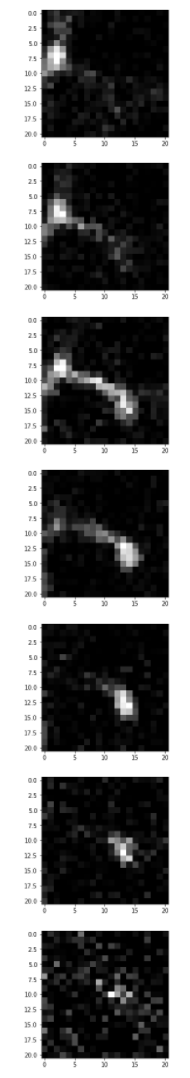
\includegraphics[width=0.13\linewidth]{neuron-slices}
  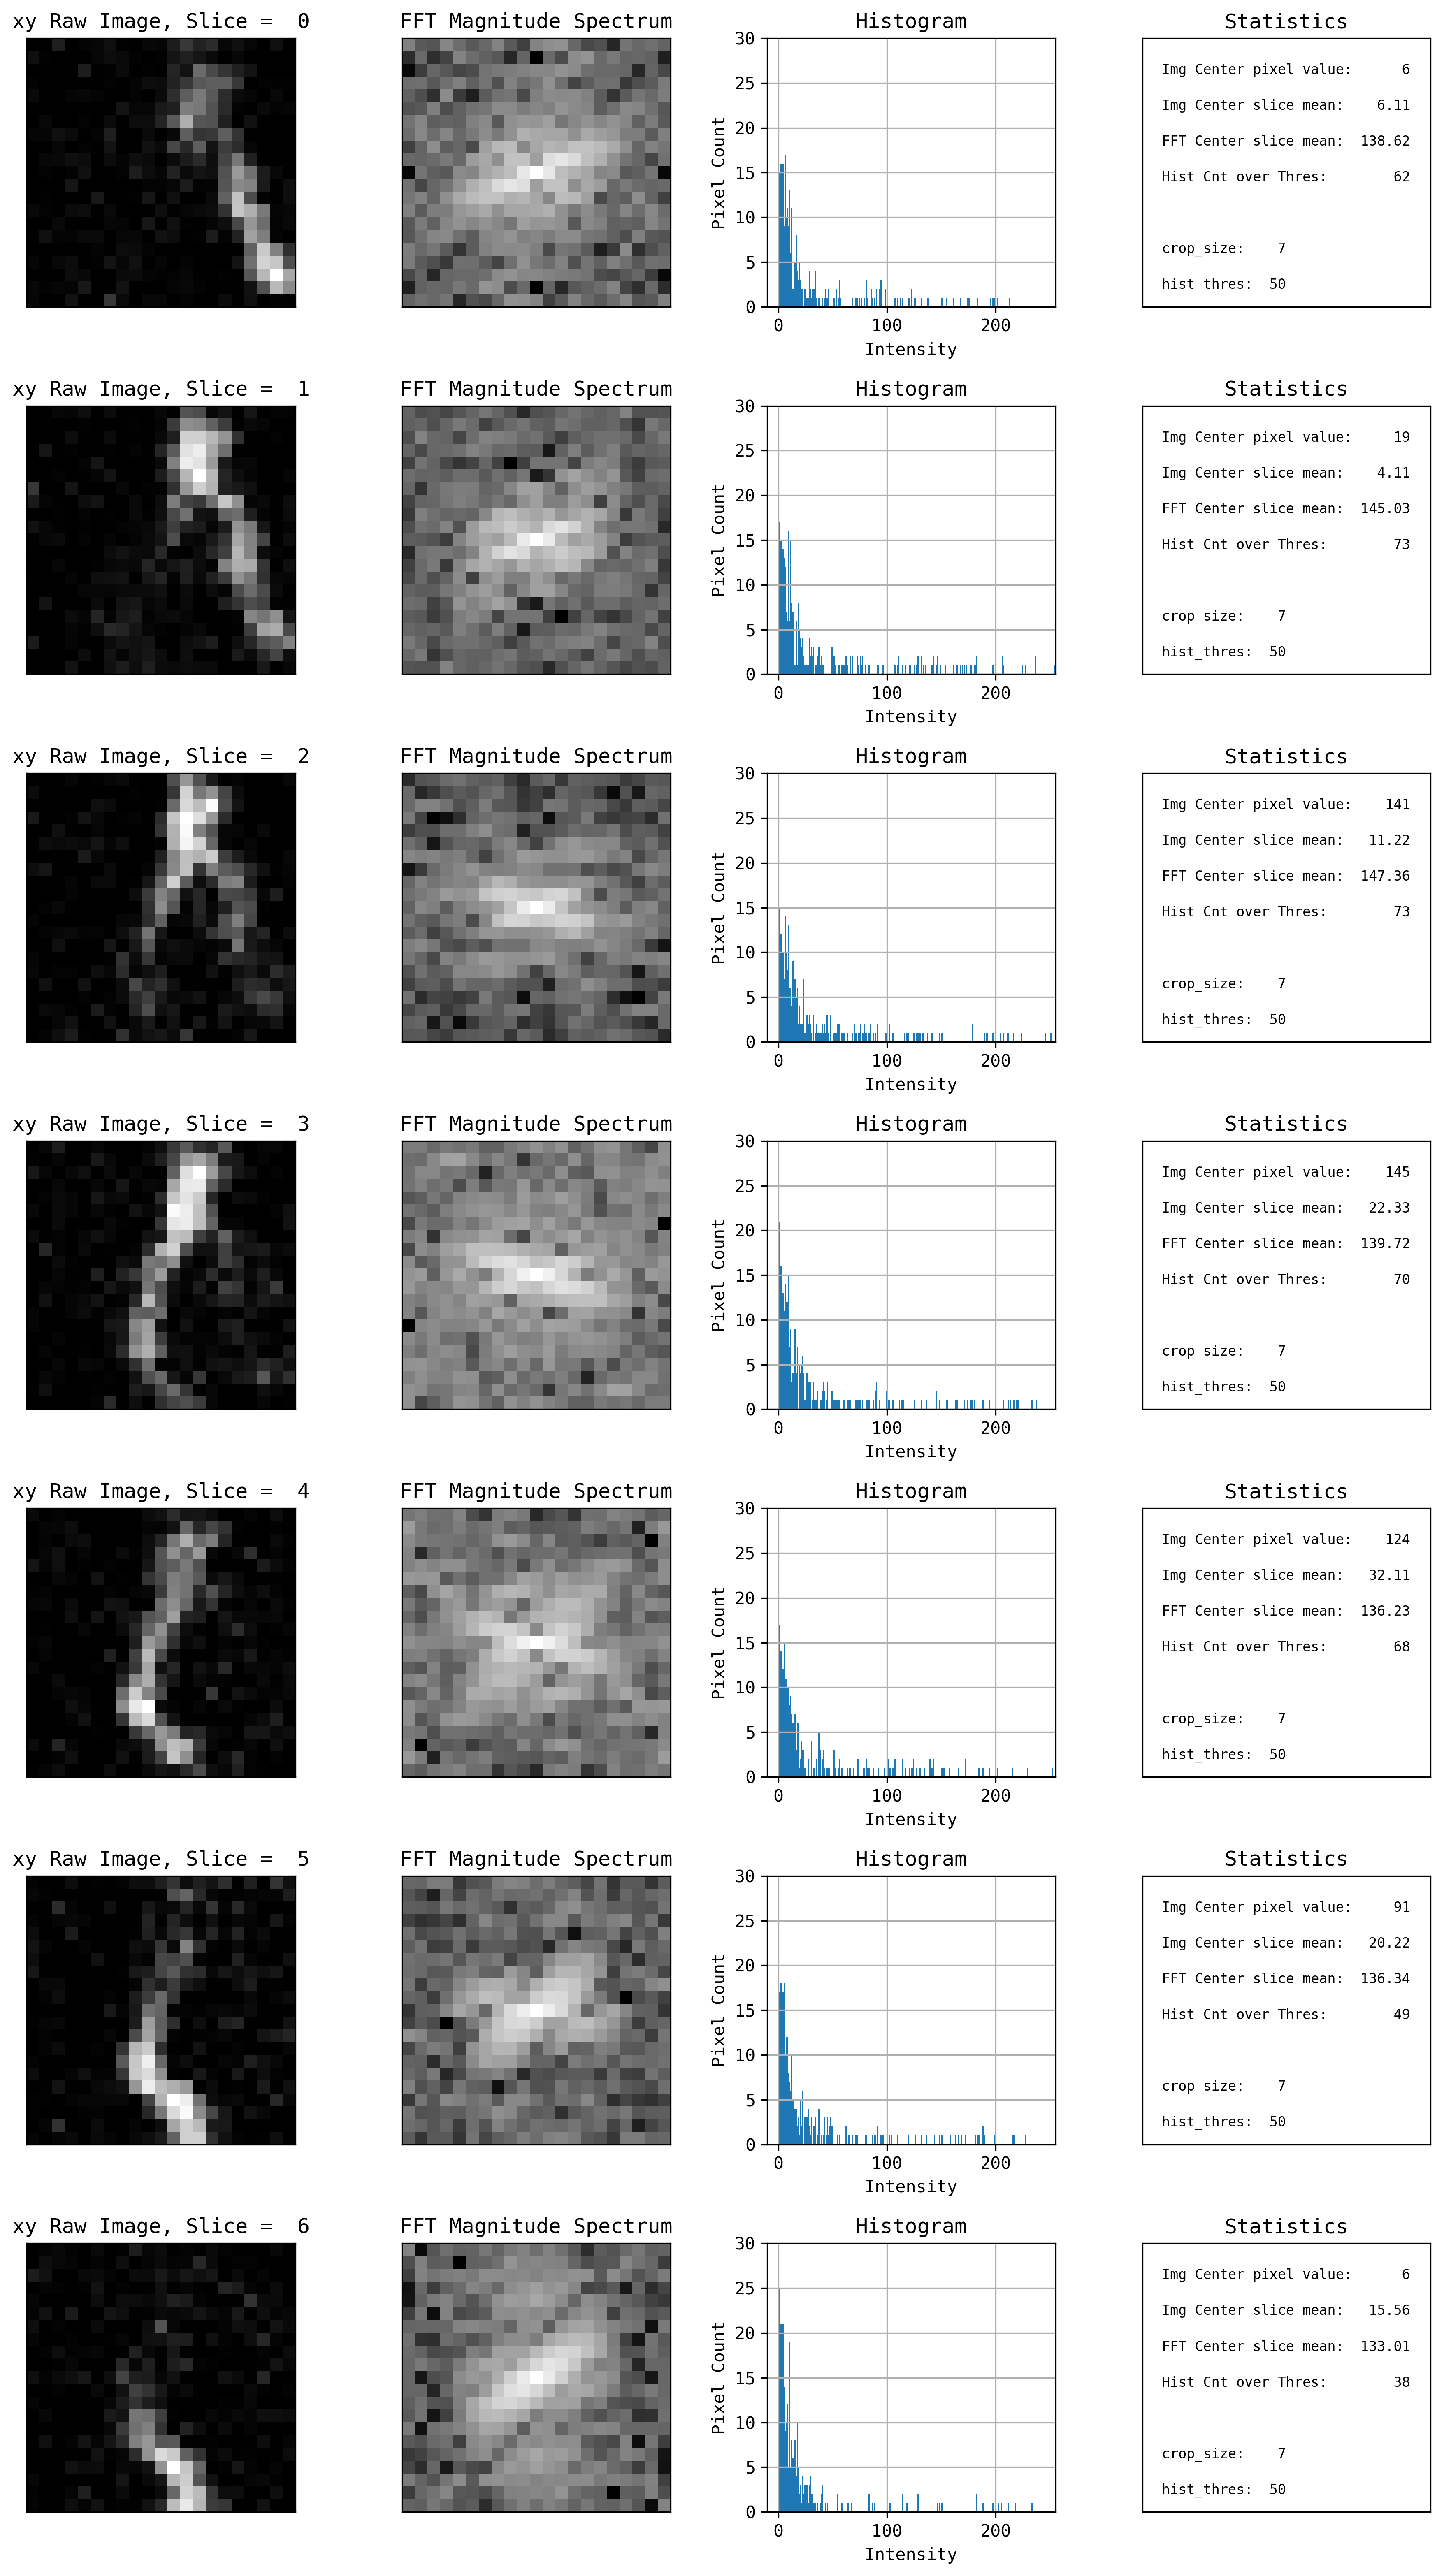
\includegraphics[width=0.42\linewidth]{foreground-xy-1}
  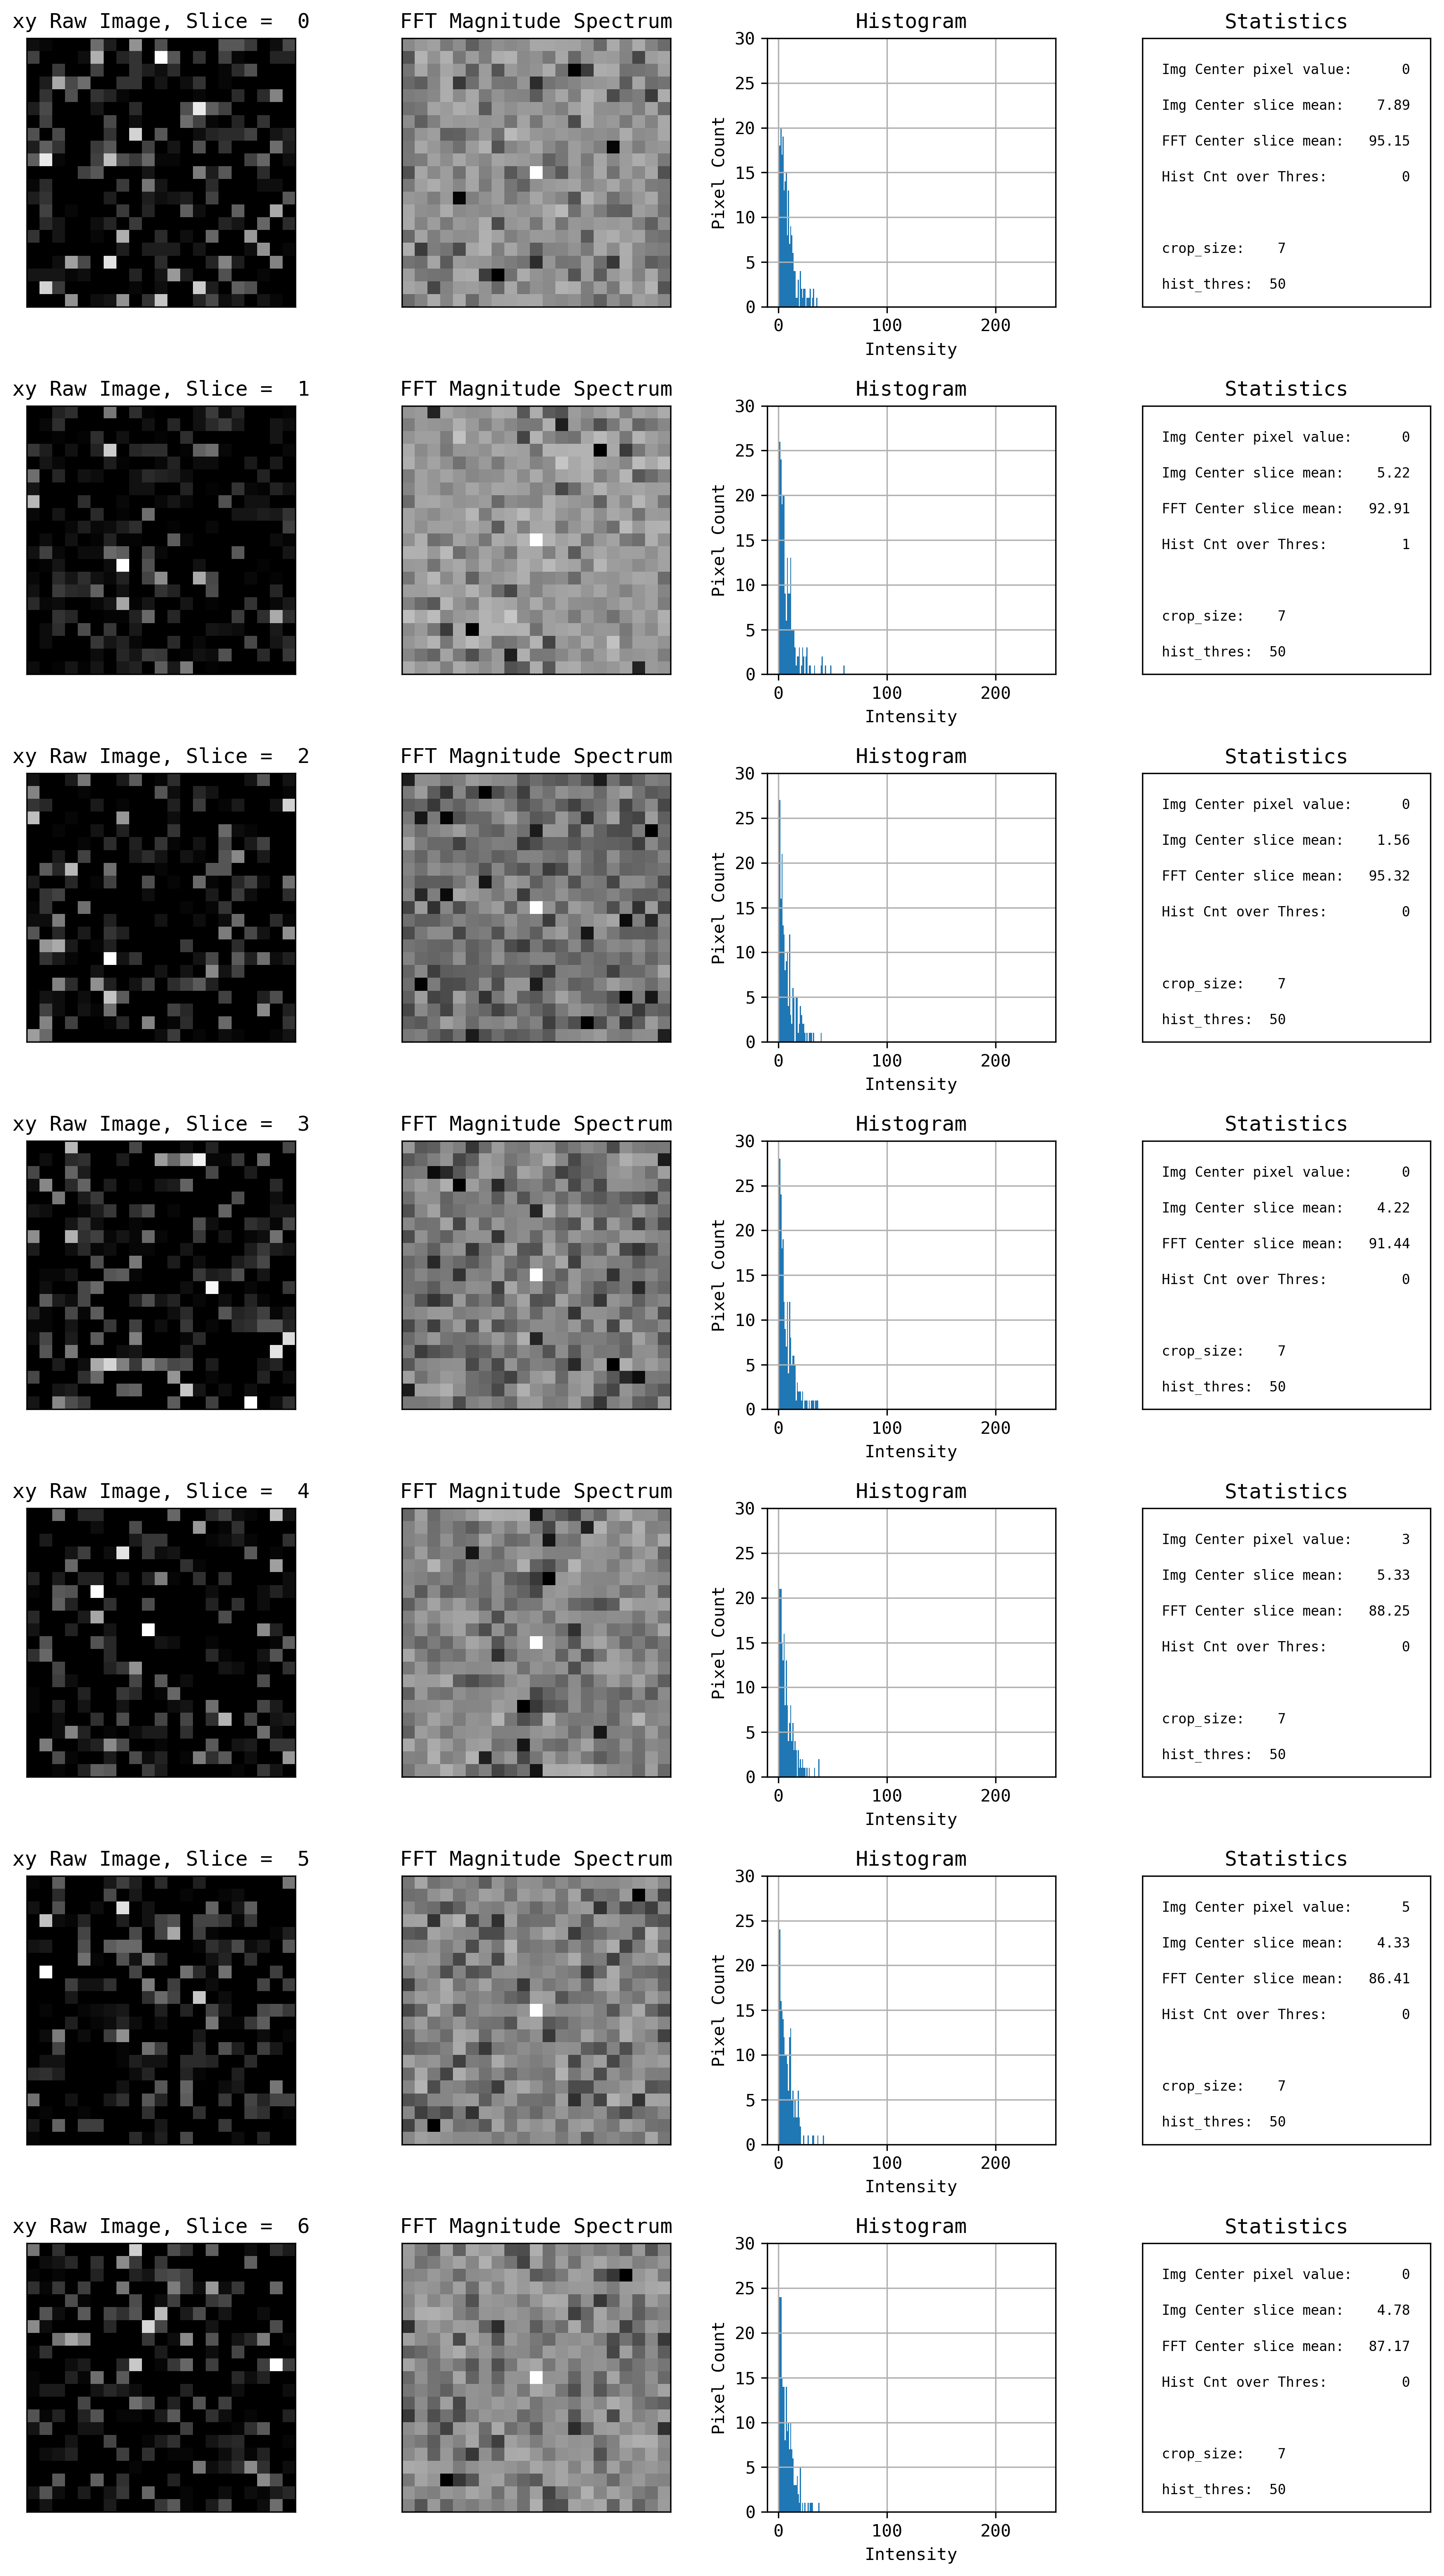
\includegraphics[width=0.42\linewidth]{background-xy-0}
  \label{fig:visualization}
\end{figure}

\section{Center Pixel - foreground and background}
\begin{figure}[!h]
  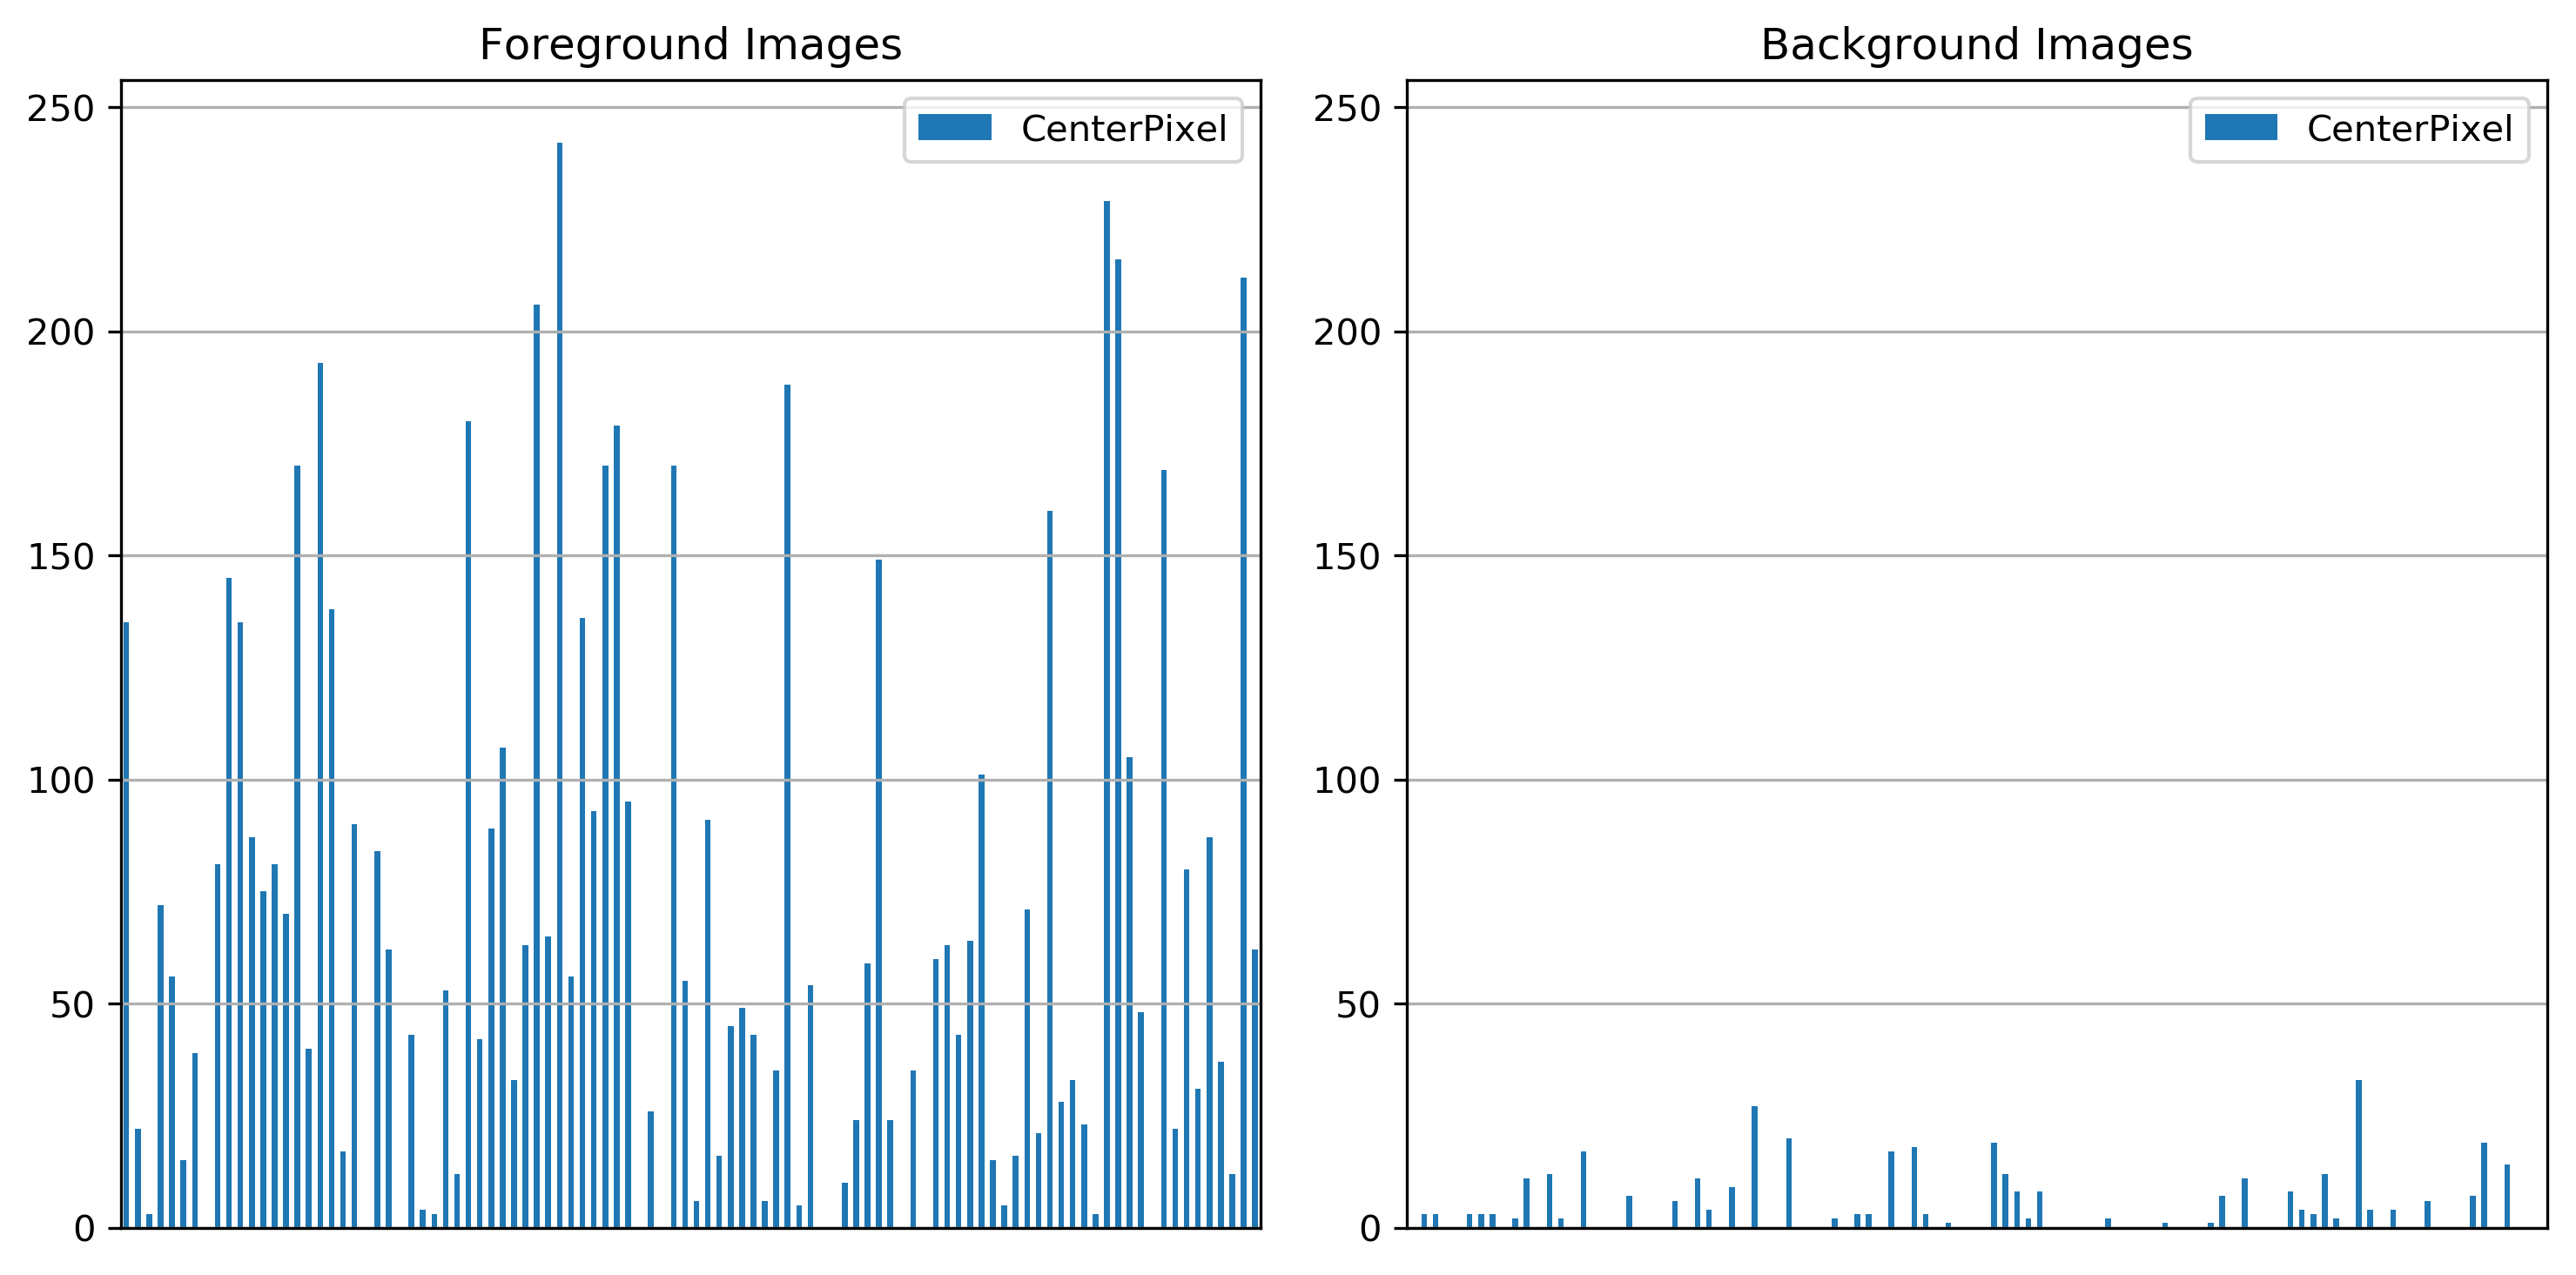
\includegraphics[width=0.6\linewidth]{feature-compare-CenterPixel}
  \label{fig:feature-compare-CenterPixel}
\end{figure}

\newpage

\section{Classification Comparison test}
\begin{figure}[!h]
  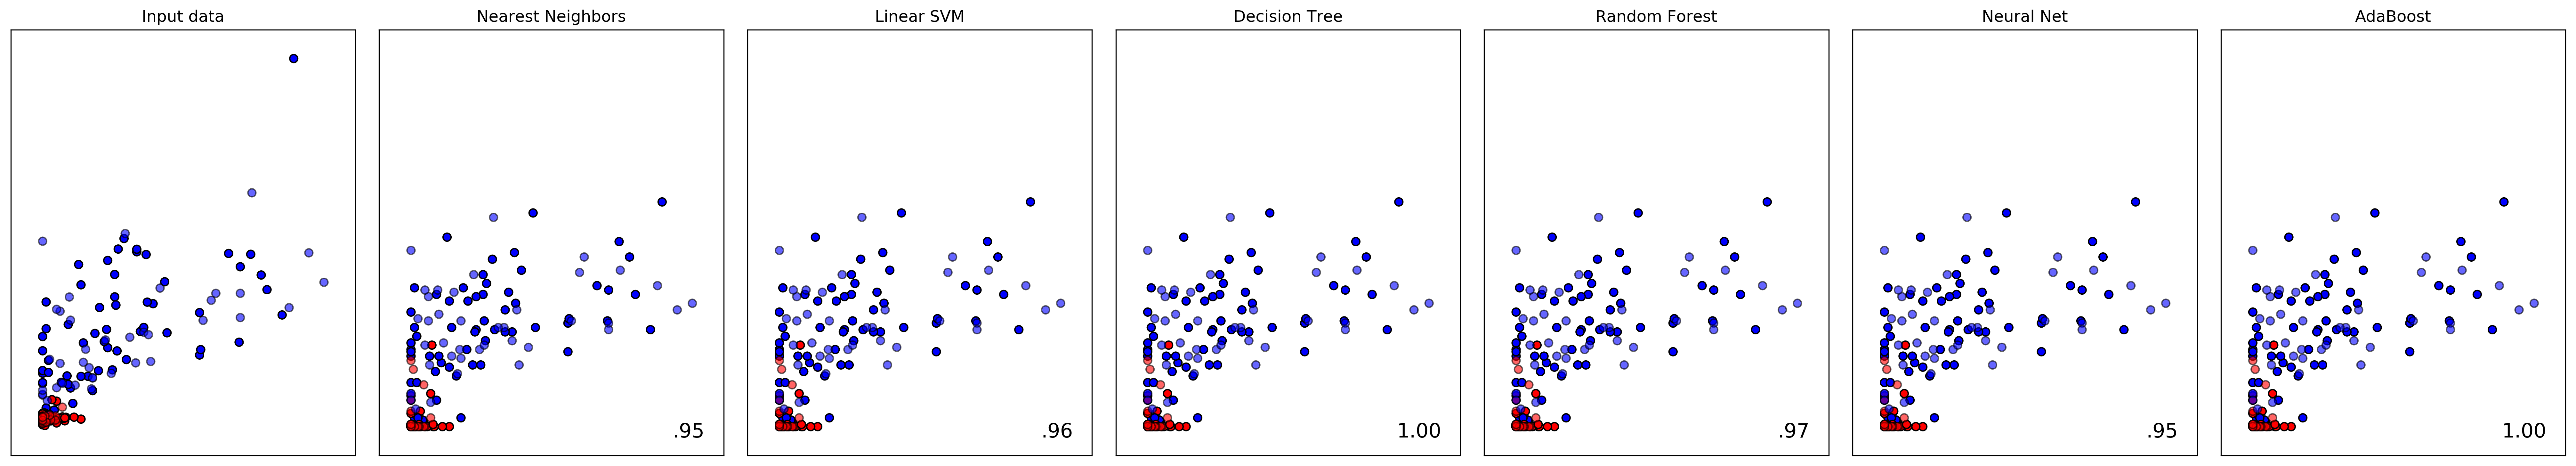
\includegraphics[width=1\linewidth]{classification-test}
  \label{fig:classification-test}
\end{figure}

\section{Application Pipeline}
\begin{figure}[!h]
  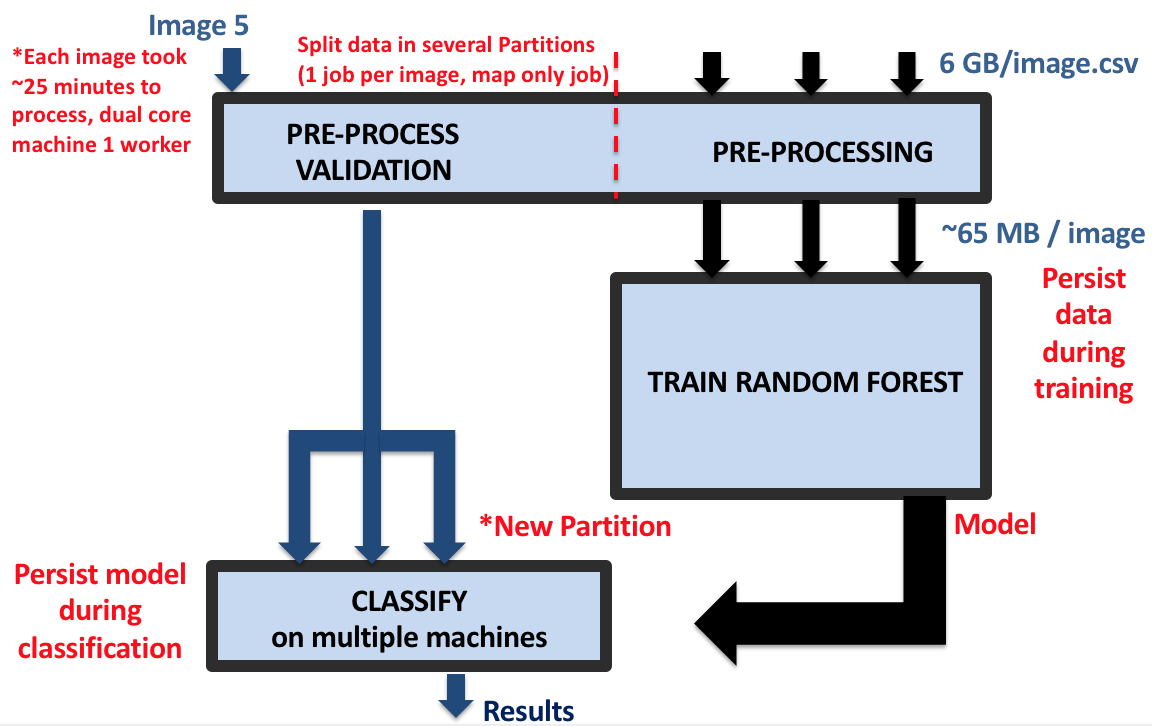
\includegraphics[width=0.7\linewidth]{pipeline}
  \label{fig:pipeline}
\end{figure}




\end{document}
